\documentclass[12pt,a4paper]{scrartcl}
\usepackage[brazil]{babel}
\usepackage[T1]{fontenc}
\usepackage[utf8]{inputenc}
\usepackage[onehalfspacing]{setspace}
\usepackage{graphicx}
\usepackage{hyperref}

\usepackage{amssymb,amsfonts,amsmath,amsthm}
\usepackage{mathtools}
\usepackage{latexsym}
\usepackage[brazilian]{cleveref}

\usepackage{float}
\usepackage[table]{xcolor}
\usepackage{indentfirst}
\usepackage{dsfont}
\usepackage{caption}
\usepackage{subcaption}

\DeclareMathOperator{\proj}{proj}
\DeclareMathOperator*{\argmax}{arg\, max}
\DeclareMathOperator*{\argmin}{arg\, min}
\DeclareMathOperator{\diag}{diag}
\DeclareMathOperator{\ones}{ones}

\def\Xset{\mathcal{X}}
\def\Yset{\mathcal{Y}}
\def\Hset{\mathcal{H}}
\def\RR{\mathds{R}}
\def\xbar{\bar{x}}
\def\wbar{\bar{w}}
\def\bbar{\bar{b}}


\newtheorem{teorema}{Teorema}%ambientes em itálico
\newtheorem{prop}{Proposição}
\newtheorem{teo}{Teorema}
\newtheorem{lema}{Lema}

\theoremstyle{definition}%ambientes normais
\newtheorem{exem}{Exemplo}[subsection]
\newtheorem{defi}{Definição}

\usepackage{csquotes}
\usepackage[
backend=biber,
style=numeric-comp, noerroretextools=true
]{biblatex}
\addbibresource{referencias.bib}

 \let\etoolboxforlistloop\forlistloop % save the good meaning of \forlistloop
 \usepackage{autonum}
 \let\forlistloop\etoolboxforlistloop % restore the good meaning of \forlistloop
 
 
\begin{document}

\title{Análise Teórica de Máquinas de Vetores Suporte} 
\author{ \normalfont Aluna: Paula Cristina Rohr Ertel \\ \normalfont Orientador: Luiz Rafael dos Santos \\ \normalfont Universidade Federal de Santa Catarina - Campus Blumenau}
\date{18 de Novembro de 2019}
\maketitle
\section{Introdução à SVM}

A Aprendizagem de Máquina (do inglês \textit{Machine Learning}) é o estudo do uso de técnicas computacionais para automaticamente detectar padrões em dados e usá-los para fazer predições e tomar decisões. De acordo com \textcite{Evelin2017}, existem dois tipos de Aprendizagem de Máquina, a aprendizagem supervisionada, em que a partir de um conjunto de dados de entrada e saída a máquina constrói um modelo que deduz a saída para novas entradas, e a não supervisionada, na qual a máquina cria sua própria solução. 

A aprendizagem supervisionada é composta por uma etapa denominada fase de treinamento, na qual é dado um conjunto de treinamento formado por vários dados de entrada e saída que funcionam como exemplos, a partir dos quais a máquina detecta padrões e cria um modelo para deduzir a saída de novos dados. Após essa fase novas entradas são testadas, denominadas conjunto de teste, no intuito de analisar se a máquina está gerando as saídas corretas. Algumas técnicas para aprendizagem de máquina supervisionada são as Máquinas de Vetores Suporte, Regressão Linear, Regressão Logística e Redes Neurais. Enquanto que a \textit{Singular Value Decomposition} (SVD), Clusterização e Análise de Componentes Principais \cite{Evelin2017} são exemplos de técnicas para a aprendizagem não supervisionada. 

As Máquinas de Vetores Suporte (SVM, do inglês \textit{Support Vector Machine}), conforme mencionado por \textcite{Evelin2017}, são indicadas nos casos em que ocorrem dados de dimensões elevadas e com altos níveis de ruídos, além de apresentar uma boa capacidade de generalização. Esta técnica pode ser aplicada tanto para problemas de regressão como de classificação. Segundo \textcite{Evelin2017}, essa técnica foi desenvolvida por Vladimir Vapnik, Bernhard Boser, Isabelle Guyon e Corrina Cortes, com base na Teoria de Aprendizagem Estatística. Algumas aplicações de SVM em problemas práticos são o reconhecimento facial, leitura de placas automotivas e detecção de spam.


\subsection{Objetivos}

Desenvolver um estudo teórico das Máquinas de Vetores Suporte, em particular, estudar a SVM para o problema de classificação, abordando inicialmente o problema de classificação binária, isto é, quando o conjunto de valores possíveis que a classe de saída pode atingir é binário. Para tanto, neste trabalho o conjunto de saída será denotado por $\{1,-1\}$. Entretanto, quaisquer dois valores distintos poderiam ser utilizados, como $\{0,1\}$, $\{True, False\}$, $\{red, blue\}$.  

%Em muitas situações queremos que o nosso algoritmo de aprendizado de máquina preveja uma dentre várias saídas possíveis. Um exemplo, como apresentado por \textcite{Faisal2019}, é o telescópio, o qual identifica se um objeto no céu noturno é uma galáxia, uma estrela ou um planeta. 


\subsection{Referencial Teórico}
Primeiramente, fez-se necessário estudar os aspectos teóricos-matemáticos dos Métodos de Otimização relacionados ao aprendizado de máquina, mais especificamente os associados as Máquinas de Vetores Suporte. Para tanto, assim como proposto por \textcite{Faisal2019}, realizou-se uma revisão dos principais conceitos de Álgebra Linear e do Cálculo de Várias Variáveis relacionados ao assunto. Por conseguinte, desenvolveu-se um estudo teórico das condições de otimalidade para problemas de otimização sem restrições baseando-se em \textcite{Ademir2013}. Para dar continuidade ao desenvolvimento desse projeto será necessário estudar as condições de otimalidade para problemas com restrições, haja vista que um dos problemas que se pretende resolver trata-se de um problema de programação quadrática convexa com restrições lineares. Em vista disso, pretende-se utilizar como referência \textcite{Ana1994}, \textcite{Solodov2014,Izmailov2014} e \textcite{Ademir2013} para estudar a teoria de otimização com restrições, progamação quadrática e dualidade. O estudo específico acerca dos aspectos teóricos-matemáticos da técnica de Máquinas de Vetores Suporte será desenvolvido a partir de \textcite{Evelin2017}.


\subsection{Máquinas de Vetores Suporte - Margem Rígida}
 
Considere um conjunto de dados, pertencentes a duas classes distintas, conforme \Cref{fig1}.

\begin{figure}[!h] 
\centering
\begin{subfigure}[h]{0.3\textwidth}
\centering
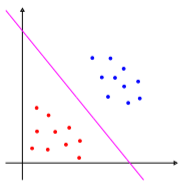
\includegraphics[width=\textwidth]{SVM_linear}
\caption{Linear. \label{fig1:a}}
\end{subfigure}
\begin{subfigure}[!h]{0.3\textwidth}
	\centering
	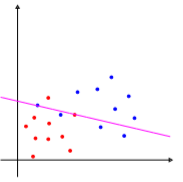
\includegraphics[width=\textwidth]{SVM_flexivel}
	\caption{Flexível. \label{fig1:b}}
\end{subfigure}
\begin{subfigure}[!h]{0.3\textwidth}
	\centering
	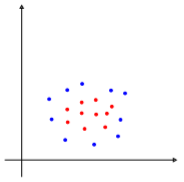
\includegraphics[width=\textwidth]{SVM_naolinear}
	\caption{Não Linear. \label{fig1:c}}
\end{subfigure}
\caption{Dados lineares, com margem flexível e não lineares. \label{fig1}\\ Fonte: \textcite{Evelin2017}}
\end{figure}

Observe que na \Cref{fig1:a} os dados podem ser classificados corretamente através de uma reta. Já na \Cref{fig1:b} é possível encontrar uma reta que separa alguns poucos dados, porém incorretamente. E na \Cref{fig1:c} não é possível classificar os dados como nos casos anteriores. Nestes exemplos temos representados os três casos de SVM: o linear com margem rígida, o linear com margem flexível e o não linear, respectivamente.

A modelagem do problema de classificação, utilizando a técnica de SVM, consiste em encontrar um hiperplano ótimo que melhor separe os dados de entrada $x^i$ em duas saídas $y_i$ através de uma função de decisão. Matematicamente, mostraremos que trata-se um problema de programação quadrática convexa com restrições lineares, que pode ser formulado como
\[
\begin{aligned}
\min_{w,b} & \quad f(w,b) \\
\text{s.a.} &  \quad g(w,b) \leq 0, \end{aligned}
\]
com $w\in \RR^n$ e $b\in \RR $, em que $f: \RR^n \rightarrow \RR$ é uma função quadrática e $g: \RR^{n+1} \rightarrow \RR^m$ é linear. Note também que $f$ e $g$ são continuamente diferenciáveis.

%envolve um problema de programação não linear, quadrático, convexo e restrito, no qual o objetivo é encontrar um hiperplano ótimo $(w^{*})^{T}x+b^{*}=0$ que separe os dados de entrada $x^{i}$ em duas classes de saída $y_{i}$. Assim, pretendemos estudar primeiramente o caso de classificação com margem rígida e posteriormente sua generalização para o caso com margem flexível. Por fim, abordaremos o problema de classificação não linear. 



Para formular matematicamente o problema de classificação, considere os conjuntos de entrada $\Xset =\{x^1, \ldots , x^m \} \subset \RR^n$ e de treinamento $\Yset=\{(x^1, y_1), \ldots , (x^m, y_m)\mid x^i \in \Xset \, e \, y_i \in \{-1,1\}\}$, com a partição 
\[ \label{conj1}
\Xset ^{+} =\{x^i \in \Xset\mid y_i=1\} \quad e \quad \Xset^{-}=\{x^i \in \Xset\mid y_i=-1\},
\]
dos conjuntos formados pelos atributos pertencentes às classes positiva e negativa, respectivamente.

\begin{defi} Considere um vetor não nulo $w\in \RR^n$ e um escalar $b\in \RR$. Um hiperplano com vetor normal $w$ e constante $b$ é um conjunto da forma $\Hset(w,b)=\{x\in \RR^n \mid w^{T}x+b=0\}$.
\end{defi}

O hiperplano $\Hset(w,b)$ divide o espaço $\RR^n$ em dois semiespaços, dados por
\[ \label{conj2}
\mathcal{S}^{+}=\{x\in \RR^n \mid w^{T}x+b\geq 0\} \quad e \quad \mathcal{S}^{-}=\{x\in \RR^n \mid w^{T}x+b\leq 0\}.
\]

Considere dois conjuntos de dados de treinamento representados no $\RR^2$ como na \Cref{fig2:a}, em que os pontos em azul representam a classe positiva, e os pontos em vermelho a classe negativa. Perceba na \Cref{fig2:b} que todos os hiperplanos representados separam corretamente os dados, porém nosso objetivo será encontrar o hiperplano que melhor separa esses dados, o qual está representado na \Cref{fig3:a} pela cor violeta. Logo, desejamos encontrar o hiperplano que possibilita a maior faixa que não contém nenhum dado, pois caso a faixa seja muito estreita pequenas perturbações no hiperplano ou no conjunto de dados podem resultar uma classificação incorreta. 
\begin{figure}[htbp] 
	\centering
	\begin{subfigure}[h]{0.4\textwidth}
		\centering
		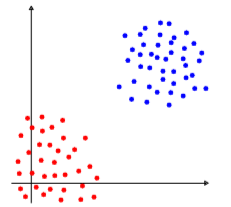
\includegraphics[width=\textwidth]{dados_treinamento}
		\caption{Dados de treinamento. \label{fig2:a}}
	\end{subfigure}
	\begin{subfigure}[h]{0.38\textwidth}
		\centering
		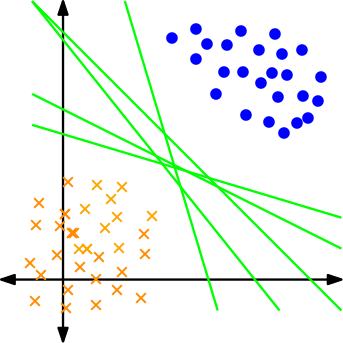
\includegraphics[width=\textwidth]{hiperplanos_separadores}
		\caption{Hiperplanos separadores. \label{fig2:b}}
	\end{subfigure}
\caption{Conjunto de Dados e Hiperplanos. \label{fig2}
	\\ Fonte: \textcite{Evelin2017}}
\end{figure}
\begin{figure}[hbtp] 
	\centering
	\begin{subfigure}[h]{0.38\textwidth}
		\centering
		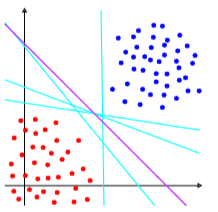
\includegraphics[width=\textwidth]{hiperplano_otimo}
		\caption{Hiperplano ótimo. \label{fig3:a}}
	\end{subfigure}
	\begin{subfigure}[h]{0.38\textwidth}
		\centering
		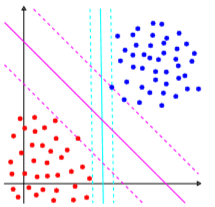
\includegraphics[width=\textwidth]{maxima_margem}
		\caption{Máxima margem. \label{fig3:b}}	
	\end{subfigure}
\caption{Hiperplano Ótimo. \label{fig3}
\\ Fonte: \textcite{Evelin2017}}
\end{figure}

\begin{defi} \label{def1} Os conjuntos $\Xset^{+}, \Xset^{-} \subset \RR^n$ são ditos linearmente separáveis quando existem $w\in \RR^n$ e $b\in \RR$  tais que $w^{T}x+b>0$ para todo $x\in \Xset^{+}$ e $w^{T}x+b<0$ para todo $x\in \Xset^{-}$. O hiperplano $\Hset(w,b)$ é chamado hiperplano separador dos conjuntos $\Xset^{+}$ e $\Xset^{-}$.
\end{defi}

\begin{lema} \label{lema1} Suponha que os conjuntos $\Xset^{+}, \Xset^{-} \subset \RR^n$ são finitos e linearmente separáveis, com hiperplano separador $\Hset(w,b)$. Então, existem $\overline{w}\in \RR^n$ e $\overline{b}\in \RR$ tais que $\Hset(w,b)$ pode ser descrito por
\[
\wbar^{T}x+\bbar =0,
\]
satisfazendo
\begin{align}
\wbar^{T}x+\bbar &\geq 1, \text{ para todo } x\in \Xset^{+}, \label{eq1} \\
\wbar^{T}x+\bbar &\leq -1, \text{ para todo } x\in \Xset^{-}. \label{eq2}
\end{align}
\end{lema} 

\begin{proof}
Pela  \Cref{def1}, temos que existem $w\in \RR^n$ e $b\in \RR$ tais que
\begin{align}
w^{T}x+b &>0, \text{ para todo } x\in \Xset^{+}, \\
w^{T}x+b &<0, \text{ para todo } x\in \Xset^{-}.
\end{align}  

Como $\Xset^{+}\cup \Xset^{-}$ é um conjunto finito, podemos definir
\[ \gamma \coloneqq \min_{x\in \Xset^{+}\cup \Xset^{-}} \vert w^{T}x+b\vert  >0. \]

Portanto, para todo $x\in \Xset^{+}\cup \Xset^{-}$, $\gamma \leq \vert w^{T}x+b\vert$ e consequentemente, $\dfrac{\vert w^{T}x+b\vert }{\gamma} \geq 1$. Assim, para $x\in \Xset^{+}$ temos
\[ \dfrac{w^{T}x+b}{\gamma} = \dfrac{\vert w^{T}x+b\vert }{\gamma} \geq 1, \]
e para $x\in \Xset^{-}$, temos
\[- \dfrac{w^{T}x+b}{\gamma} = \dfrac{\vert w^{T}x+b\vert }{\gamma} \geq 1. \]

Logo, definindo $\wbar:=\dfrac{w}{\gamma}$ e $\bbar :=\dfrac{b}{\gamma}$, obtemos as desigualdades \eqref{eq1} e \eqref{eq2}. 

\end{proof}

A partir do \Cref{lema1} temos que $\Hset^{+}:=\{x\in \RR^n \mid w^{T}x+b= 1\}$ e $\Hset^{-}:=\{x\in \RR^n \mid w^{T}x+b= -1\}$ são os hiperplanos que definem a faixa que separa os conjuntos $\Xset^{+}$ e $\Xset^{-}$.

\begin{prop} \label{prop1} A projeção ortogonal de um vetor $\xbar\in \RR^n$ sobre um hiperplano afim $\Hset(w,b)$, é dada por
\[ \proj_{\Hset}(\xbar)= \xbar - \dfrac{w^{T}\xbar+b}{w^{T}w}w. \]
Além disso, a $\proj_{\Hset}(\xbar)$ satisfaz a menor distância.
\end{prop}

\begin{proof}
Sejam $w\in \RR^n$ o vetor normal ao hiperplano $\Hset(w,b)$, $\bar{z}\in \Hset(w,b)$ e $x^{*}$ a projeção ortogonal de $\xbar$ sobre $\Hset(w,b)$. Assim, temos que 
\[ \label{eq3} w^{T}(x^{*}-\bar{z})=0 \]
e
\[ \label{eq4} \xbar-x^{*}=\lambda w \Longrightarrow x^{*}=\xbar-\lambda w. \]

Substituindo \eqref{eq4} em \eqref{eq3}, obtemos
\begin{align}
0 &= w^{T}(\xbar-\lambda w-\overline{z}) \\
&= w^{T}\xbar-\lambda w^{T}w - w^{T}\bar{z}.
\end{align}

Resolvendo para $\lambda$ e como $w^{T}\bar{z} = -b$, temos
\[ \lambda =\dfrac{w^{T}\xbar-w^{T}\bar{z}}{w^{T}w} =\dfrac{w^{T}\xbar+b}{w^{T}w}. \]

Portanto, 
\[ x^{*}=\xbar-\dfrac{w^{T}\xbar+b}{w^{T}w}w . \]

Ademais, vamos provar que a $\proj_{\Hset}(\xbar)$ satisfaz a menor distância, isto é,
\[ \Vert\xbar-x^{*}\Vert_{2} \leq \Vert \xbar-x\Vert_{2}, \]
para todo $x\in \Hset(w,b)$.

De fato, tomando $u=\xbar-x^{*}$ e $v=x^{*}-x$ observe que 
\begin{align}
u^{T}v&= (\xbar-x^{*})^{T}(x^{*}-x) \\
&= (\xbar-\xbar+\lambda w)^{T}(x^{*}-x) \\
&= \lambda w^{T}(x^{*}-x) \\
&= \lambda (w^{T}x^{*}-w^{T}x) \\
&= \lambda (-b-(-b)) \\
&= 0.
\end{align}

Assim, temos
\[ \Vert u+v\Vert^{2}=\Vert u\Vert^{2} + 2u^{T}v + \Vert v\Vert^{2}=\Vert u\Vert^{2} + \Vert v\Vert^{2} , \]
ou seja,
\[ \Vert \xbar-x\Vert^{2}=\Vert \xbar-x^{*}\Vert^{2} + \Vert x^{*}-x\Vert^{2}. \]

\end{proof}

Utilizando a \Cref{prop1} podemos demonstrar o \Cref{lema2}, o qual estabelece a largura da faixa entre os hiperplanos separadores $\Hset^{+}$ e $\Hset^{-}$.

\begin{lema} \label{lema2} A distância entre os hiperplanos $\Hset^{+}$ e $\Hset^{-}$ é dada por $d=\dfrac{2}{\Vert w\Vert}$. 
\end{lema}
\begin{proof}
Considere um ponto arbitrário $\xbar\in \Hset^{+}$ e seja $x^{*}\in \Hset^{-}$ a projeção ortogonal de $\xbar$ sobre $\Hset^{-}$. Usando a \Cref{prop1}, temos
\[ \label{eq6} x^{*}= \proj_{\Hset^{-}}(\xbar)= \xbar - \dfrac{w^{T}\xbar+b+1}{\Vert w\Vert^{2}}w. \] 

Além disso, a distância entre dois conjuntos é definida por
\[ d(\Hset^{+}, \Hset^{-}):= \inf\{\Vert x^{+}-x^{-} \Vert : x^{+}\in \Hset^{+} \ \text{e} \ x^{-}\in \Hset^{-}\},
\]
e como a $\proj_{\Hset^{-}}(\xbar)$ satisfaz a menor distância entre $\xbar$ e $\Hset^{-}$, e $\Hset^{+}$ é paralelo a $\Hset^{-}$, temos que 
\[ \label{eq7} d(\Hset^{+},\Hset^{-})=\Vert \xbar-x^{*}\Vert. \]

Substituindo \eqref{eq6} em \eqref{eq7} obtemos
\begin{align} 
d(\Hset^{+},\Hset^{-}) &= \Vert \xbar-x^{*}\Vert \\
&= \Vert \xbar -\xbar +\dfrac{w^{T}\xbar+b+1}{\Vert w\Vert^{2}}w \Vert \\
&=  \dfrac{\vert w^{T}\xbar+b+1 \vert}{\Vert w\Vert^{2}} \Vert w\Vert \\
&= \dfrac{\vert w^{T}\xbar+b+1 \vert}{\Vert w\Vert},
\end{align}
e como $\xbar\in \Hset^{+}$,  $ w^{T}\xbar+b=1$ implica
\[  w^{T}\xbar =1-b, \]
concluindo que 
\begin{align} 
d(\Hset^{+},\Hset^{-})&= \dfrac{\vert 1-b+b+1 \vert}{\Vert w\Vert} \\
&= \dfrac{2}{\Vert w\Vert }. 
\end{align}
\end{proof}

\subsection{Formulação do Problema de Classificação}

Encontrar o hiperplano que melhor separa os dados implica maximizar a largura da margem, isto é, maximizar $d=\dfrac{2}{\Vert w\Vert }$. Isso equivale a minimizar seu inverso $\dfrac{1}{2}\Vert w\Vert $ ou ainda minimizar $\dfrac{1}{2}\Vert w\Vert^{2}$. De fato, seja $w^{*}=\argmax\dfrac{2}{\Vert w\Vert}$. Então, para todo $w\in \RR^n$,
\[ \dfrac{2}{\Vert w^{*}\Vert} \geq \dfrac{2}{\Vert w\Vert} \]
implica
\[ \label{eq8} \Vert w\Vert \geq \Vert w^{*}\Vert. \]
Logo, $w^{*}=\argmin\Vert w\Vert$. Além disso, como $\Vert .\Vert$ é não negativa, elevando ao quadrado ambos os lados da desigualdade \eqref{eq8} temos que  $\Vert w\Vert^{2} \geq \Vert w^{*}\Vert^{2}$ implica
\[ \dfrac{1}{2}\Vert w\Vert^{2} \geq \dfrac{1}{2}\Vert w^{*}\Vert^{2}. \]

Portanto, 
\[ \argmax\dfrac{2}{\Vert w\Vert} = \argmin\dfrac{1}{2}\Vert w\Vert^2. \]

Ademais, como a faixa deve separar os dados das duas classes, as seguintes restrições devem ser satisfeitas
\begin{align}
w^{T}x+b &\geq 1 , \text{ para  todo } x\in \Xset^{+}, \\
w^{T}x+b &\leq -1 , \text{ para  todo } x\in \Xset^{-}.
\end{align}

Considerando que $\Xset^{+}=\{x^i \in \Xset\mid y_i=1\}$ e $\Xset^{-}=\{x^i \in \Xset \mid y_i=-1\}$, podemos reescrever as restrições acima de uma forma mais compacta 
\[ y_{i}(w^{T}x^{i}+b)\geq 1, \quad i=1, \ldots ,m. \]

Portanto, o problema de encontrar o hiperplano ótimo pode ser formulado da seguinte maneira
\[ \label{eq5}
\begin{aligned}
\min_{w,b} & \quad \dfrac{1}{2} \Vert w\Vert^{2} \\
\text{s.a.} &  \quad y_i(w^{T}x^{i}+b) \geq 1, \quad i=1, \ldots , m, \end{aligned}
 \]
em que $w\in \RR^{n}$ e $b\in \RR$. 

O problema \eqref{eq5} possui função objetivo 
\[ f(w,b)=\dfrac{1}{2}\Vert w\Vert^{2} \]
convexa, e restrições lineares
\[ g_i(w,b)=1-y_i(w^{T}x^{i}+b) \leq 0, \quad i=1, \ldots, m, \]
em que a função $g:\RR^{n+1} \rightarrow \RR^{m}$ pode ser escrita da forma 
\[ g(w,b)= e - (YX^{T}w+by) \leq 0, \]
com $e$ sendo o vetor cujas $m$ componentes são todas iguais a $1$, $Y=\diag(y_{i})$, $X=\diag(x^{i})$, $y^{T}=[y_{1} \ \ldots \ y_{m}]$, $w\in \RR^n$ e $b\in \RR$.

\section{Projetos Futuros}
O problema de classificação utilizando a técnica de SVM trata-se de um problema de programação quadrática convexa com restrições lineares. Para dar continuidade ao projeto será necessário estudar a teoria de otimização com restrições e a teoria de dualidade, em particular a relacionada ao problema de programação quadrática com restrições lineares. Por fim, pretendemos realizar uma pequena implementação computacional da técnica de Máquinas de Vetores Suporte a um problema de classificação. Para tanto, utilizaremos a linguagem de programação \texttt{Julia}, sobre a qual também será preciso estudar e se aperfeiçoar.


\printbibliography
\end{document}